%%
%% Modified by Ricardo Garcia-Rosas to satisfy the rules established by the University of Melbourne's Research Higher Degrees Committee as of 4th of June 2019.
%% Guidelines can be found at: https://gradresearch.unimelb.edu.au/__data/assets/pdf_file/0004/2027839/Preparation-of-GR-theses-rules.pdf
%%

\documentclass[a4paper, 11pt, oneside]{proposal}  

\graphicspath{figures/} 

\usepackage[square, numbers, comma, sort&compress]{natbib} 
\usepackage{graphicx}
\usepackage{caption}
\usepackage{subcaption}
\usepackage{verbatim} 
\usepackage{vector} 
\usepackage{listings} 
\usepackage{amsmath, amsfonts}
\usepackage{bussproofs}
\usepackage{tabularx}
% \setlength {\marginparwidth }{2cm}\usepackage{todonotes}
\usepackage{tipa}
\usepackage{tikz}
\usepackage{varwidth}
\usepackage[trace]{iexec}
\usepackage{pgfgantt}

\usetikzlibrary{chains,shapes,arrows,calc}
\tikzstyle{line} = [draw, -latex']
\tikzstyle{box} = [rectangle, draw=black!50, align=left, font={\ttfamily}]
\tikzstyle{init} = [circle, draw=black!50]

\hypersetup{urlcolor=blue, colorlinks=true} 

\begin{document}
\frontmatter 

\UNIVERSITY{{THE UNIVERSITY OF MELBOURNE }}    
\department{{Department of Computing and Information Systems}}
\school{{Melbourne School of Engineering \& IT}}

\degree{Master of Computer Science}
\title  {Research Proposal for Higher order programming in Wybe}
\shortauthors{James Barnes}
\authors  {\texorpdfstring
            {\href{mailto:barnesj2@student.unimelb.edu.au}{\shortauthornames}}
            {\shortauthornames}\\ 
            \small Student Number: 820946
            }
\supervisor{Peter Schachte}
\addresses  {\groupname\\\deptname\\ \univname} 
\date       {\today}
\subject    {}
\keywords   {}
%TC:ignore
\wordcount  {\iexec[\jobname-wc.tmp]{texcount -q -inc -merge -1 -sum \jobname.tex}}
% texcount ./proposal/proposal.tex -merge -1 -sum -dir=proposal
%TC:endignore

\maketitle

\setstretch{1.3} 

\fancyhead{} 
\rhead{\thepage} 
\lhead{}

\pagestyle{fancy} 

\setstretch{1.3}

%TC:ignore

\addtotoc{Abstract}  
\abstract{
\addtocontents{toc}{\vspace{1em}} 

Higher-order programming allows for a greater level of abstraction over first-order programming. Allowing for procedures to be passed into or out of a procedure is the hallmark of this programming style. An emerging programming language, Wybe, currently does not support higher order programming, nor does the intermediate representation used internally by the Wybe compiler, logic programming virtual machine (LPVM). In this research, we propose an extension to LPVM, and further to Wybe, to support higher order programming. Wybe presents novel language features, which together with higher order programming, provide a novel language implementation space.

}

%TC:endignore

\clearpage 

\acknowledgements{
  I would like to acknowledge the people of the Kulin nations, the traditional custodians of the lands on which this work was produced, particularly the Wurundjeri and Wathaurong people, whose lands I both work on and reside in. I pay my respects to the elders, past, present, and future.

  I would also like to acknowledge the assistance lent to me by my supervisor, \supname. His continued guidance of me throughout this learning journey is greatly appreciated, and his wealth of knowledge and insight has been priceless. The time lent to me to talk through problems faced throughout the production of this work is greatly appreciated.

  Finally, I would like to acknowledge the support I have received from my family, partner, and friends throughout this degree. Their support through this process has been a wealth of comfort.
}

\clearpage

\clearpage 

\pagestyle{fancy}

\lhead{\emph{Contents}} 
\tableofcontents 

\addtocontents{toc}{\vspace{1em}}

\mainmatter	  
\pagestyle{fancy}  
\setstretch{1.5} 

\clearpage 

\def\chaptertitle{Introduction}

\lhead{\emph{\chaptertitle}}

\chapter{\chaptertitle}
\label{ch:intro}

This research proposal is primarily concerned with an extension to an emerging programming language, Wybe~\cite{schachte2015wybe} (pronounced \textipa{["wib\textschwa]}, \textsc{Wee-Buh}), to extend the language to support higher order programming. Wybe is intended to be a language that teaches principled programming practices from learning through to practice.

A defining feature of Wybe is a strong emphasis on interface integrity. Interface integrity refers to the property that all possible effects of a procedure are known from the interface alone, without the requirement to delve into finer-grained implementation details.

The type system of Wybe currently supports overloading based on type and mode of the arguments of a given procedure. Overloading refers to the ability to use the same name for multiple different implementations. Overloading of modes allows procedures to be executed ``in reverse'', with arguments allowed to be input or output, depending on how the procedure is called. Modes are typical of logic languages such as Prolog~\cite{colmerauer1996birth}, however are presented differently in Wybe by allowing for explicit overloading of modes. Wybe also supports generic, or polymorphic, types. 

%TC:ignore
\begin{figure}[ht]
  \centering
  \begin{varwidth}{\linewidth}
    \begin{verbatim}
def add( x:int,  y:int, ?z:int) { ?z = x + y } 
def add( x:int, ?y:int,  z:int) { ?y = z - x }
def add(?x:int,  y:int,  z:int) { ?x = z - y }

?a = 1; ?b = 2
add(a, b, ?c) # binds c to a + b
add(a, ?d, c) # binds d to c - a
\end{verbatim}
  \end{varwidth}
  \caption{An example Wybe program showing the use of multiple modes. Outputs are marked with a preceding \texttt{?}, and inputs are unmarked.}
  \label{fig:wybe-mode-example}
\end{figure}
%TC:endignore

Wybe employs a novel message passing mechanism called resources. A resource allows data to be passed by name rather than position. They are intended to be used as a parameter that is unique in a computation and also widely used, being threaded between resourceful procedure calls automatically. The quintessential example of a resource in Wybe is the \texttt{io} resource. \texttt{io} represents the state of the outside world, providing a declarative interface for input/output operations. Each call to a procedure that uses the \texttt{io} resource ensures that a change to the ``state'' of the outside world is represented as a change in the \texttt{io} resource. Other examples of resources are the program arguments vector and count, \texttt{argv} and \texttt{argc}, respectively.

%TC:ignore
\begin{figure}[ht]
  \centering
  \begin{varwidth}{\linewidth}
    \begin{verbatim}
def print_sum(a:int, b:int) use !io {
    ?c = a + b
    !print(a); !print(" + "); !print(b)
    !print(" = "); !println(c)
}

!print_sum(a, b)
\end{verbatim}
  \end{varwidth}
  \caption{An example Wybe program showing use of the \texttt{io} resource. Calls to resourceful procedures, such as \texttt{print} are marked by a preceding \texttt{!}.}
  \label{fig:wybe-resource-example}
\end{figure}
%TC:endignore

Unlike many other languages (such as Haskell~\cite{jones2003haskell}, and Java~\cite{mazinanian2017understanding}), Wybe does not support higher order functions or procedures. That is, functions or procedures are only able to pass parameters that are first order. Higher order functions allow for code to be written at a greater level of abstraction than first order code and allows for code to be written in a distinct and principled manner that is not possible with first order code. This limits the utility and expressiveness of the Wybe language.

The Wybe compiler, \texttt{wybemk}, employs a novel intermediate representation for its initial transformation and analyses phase, logic programming virtual machine (LPVM)~\cite{gange2015horn}. Despite its name, LPVM is not a virtual machine, but an intermediate representation that makes use of restricted Horn clauses, similar to that seen in logic programming languages such as Prolog~\cite{colmerauer1996birth} and Mercury~\cite{somogyi1996execution}. With the restrictions to Horn clauses, LPVM has been shown to be an efficient intermediate representation that solves many issues in other intermediate representations seen previously.

\section{Research Questions}

The intention of this project is to explore the design and implementation of higher order types in both the LPVM intermediate representation and the Wybe programming language. Further, to ensure that higher order types in Wybe and LPVM are able to be used effectively and provide benefit to a programmer, the extended language and intermediate representation will be compared with the current implementation of both.

Motivating this proposed research, three key questions are as follows:
\begin{itemize}
  \item How can the existing LPVM implementation be extended to efficiently incorporate higher order types?
  \item Can the the existing features of the Wybe language, namely resources and different properties of procedures (such as partial procedures), be extended to support higher order types?
  \item Do these extensions allow for adequate execution when compared to the existing Wybe language and LPVM intermediate representation?
\end{itemize}

\section{Document Overview}

The structure of this research proposal is as follows. 

Firstly, a literature review (\cref{ch:lit-review}) in two sections; the first (\sref{sec:intermediate-representations}) of current intermediate representations, their relative strengths and weaknesses, and identification of extensions to a particular intermediate representation; second (\sref{sec:types}), outlines type systems and their abilities to type check programs, and higher order types and their implementation.

Following (\cref{ch:research-plan}) is a research plan, outlining the major steps towards the design and implementation of the proposed extensions to the existing LPVM and Wybe type systems, and the experimental methodology and analyses used to evaluate the effectiveness of these extensions.
 
\clearpage  

\def\chaptertitle{Literature Review}

\lhead{\emph{\chaptertitle}}

\chapter{\chaptertitle}
\label{ch:lit-review}

\section{Intermediate representations}
\label{sec:intermediate-representations}

Intermediate representations are abstract languages that exist to aid in the compilation process in a compiler, being an intermediary between source code and compiled machine code. Intermediate representations are designed to better facilitate the transformations and analyses required in compilers to produce more heavily optimised machine code or to provide guarantees about certain properties of a program. The Wybe compiler, \texttt{wybemk}, employs a novel Horn clause based intermediate representation, Logic Programming Virtual Machine (LPVM)~\cite{gange2015horn}.

\subsection{Imperative intermediate representations, and SSA and allied forms}

The intermediate representations inside the compilation process for imperative languages typically are a derivative or extension of a static single assignment (SSA) form intermediate representation. SSA form was developed by Rosen, et al.~\cite{rosen1988global}, and later popularised after an efficient algorithm was devised by Cytron, et al.~\cite{cytron1991efficiently} to transform an intermediate representation into SSA form efficiently. SSA form intermediate representations typically represent the control flow graph as a graph of basic blocks, with each block terminated by a branch to some other block. 

An intermediate representation is said to be in SSA form if each variable in a given scope is assigned exactly once. This property allows certain key analyses to be performed more efficiently. For instance, as a variable is assigned once, analyses on the lifetime of the variable are greatly simplified.

Where a variable would be reassigned in a non-SSA form intermediate representation, SSA form introduces a fresh variable which acts as the new version of the variable in later uses of the variable in the control flow graph. These fresh variables propagate naturally through a linear path in a control flow graph. However, as a block can have more than one predecessor blocks, multiple versions of a variable may be available to a block. At the start of one of these blocks, SSA form introduces a $\phi$-node to disambigaute which variable is to be used. $\phi$-nodes assign the correct version of a variable to a fresh variable within a block. In translation to machine code, these $\phi$-nodes are translated to either a move instruction or omitted if register allocation can allocate the variables to the same register. Considerable effort has been made to produce SSA forms with a minimal amount of $\phi$-nodes~\cite{cooper2001simple, braun2013simple}, as these nodes do provide some bloat within the intermediate representation, however their utility lies in annotating which blocks provide the values of variables in a given block.

%TC:ignore
\begin{figure}[h]
  \begin{minipage}[b]{0.429 \textwidth}
    \centering
    \begin{varwidth}{\linewidth}
      \begin{verbatim}
int gcd(int a, int b) {
    while (b != 0) {
        int t = b;
        b = a % t;
        a = t;
    }
    return a;
}
\end{verbatim}
    \end{varwidth}
    \caption{A GCD program in C~\cite{gange2015horn}.}
    \label{fig:gcd-c}
  \end{minipage}%
  \begin{minipage}[b]{0.57 \textwidth}
    \centering
    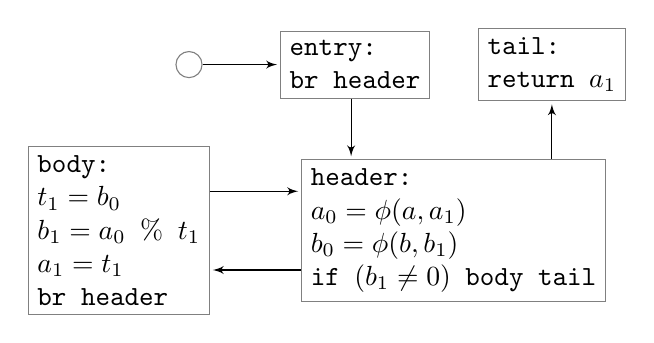
\begin{tikzpicture}[auto,
                        shorten >=1pt, 
                        node distance = 6em]
      \node [box] (header)    
        {header:\\
          $a_0 = \phi(a, a_1)$\\     
          $b_0 = \phi(b, b_1)$ \\
          if $(b_1 \neq 0)$ body tail};
      \node [box, above of=header] at (-1.25,0) (entry)    
        {entry:\\
          br header};      
      \node [init, left of=entry] (init) {};
      \node [box, above of=header] at (1.25,0) (tail)    
        {tail:\\
          return $a_1$};   
      \node [box] at (-4.25,0) (body)    
        {body:\\
          $t_1 = b_0$\\     
          $b_1 = a_0\ \%\ t_1$\\
          $a_1 = t_1$\\
          br header};
      \path [line] (init) -- (entry);
      \path [line] let \p0=($(entry.south)-(0.05,0)$), \p1=(header.north) in
        (\x0,\y0) -- (\x0,\y1);
      \path [line] let \p0=(tail.south), \p1=(header.north) in
        (\x0,\y1) -- (\x0,\y0);
      \path [line] ($(body.east)+(0,0.5)$) -- ($(header.west)+(0,0.5)$);
      \path [line] ($(header.west)-(0,0.5)$) -- ($(body.east)-(0,0.5)$);
    \end{tikzpicture}
    \caption{The GCD program in SSA form~\cite{gange2015horn}.}
    \label{fig:gcd-ssa}
  \end{minipage}
\end{figure}
%TC:endignore

In \fref{fig:gcd-ssa}, the \texttt{header} block has two possible predecessor blocks, \texttt{entry} and \texttt{body}. To disambiguate which version of $a$ and $b$ are used within the block, the two $\phi$-nodes are introduced. If the previous block in execution was \texttt{entry}, then the value of $a_0$ will be $a$, and $b_0$ will be $b$, otherwise they will be $a_1$ and $b_1$, respectively.

However, SSA form does come at a cost. $\phi$-nodes bias the representation to be amenable primarily to forward analyses. This is due to the $\phi$-nodes having no reversed dual in SSA form to indicate which branches use each variable after a branch. This effectively renders backwards value analyses infeasible, or at the very least offers much weaker analysis, as different branches may assign a different abstract value to the variable. 

This problem of forward bias of $\phi$-nodes was addressed with the addition of $\sigma$-nodes~\cite{ananian2001static} to create static single information (SSI) form. In contrast to $\phi$-nodes, $\sigma$-nodes are introduced at the end of each branching block and indicate where each variable's values are used next. This allows reasoning in both directions, eliminating the forward bias of $\phi$-nodes alone.

Even with the addition of $\sigma$-nodes in SSI form, there still exists limitations of value analyses in both SSA and SSI forms. In non-relational analysis, abstract values can propagate through $\phi$-nodes by taking the join of each abstract value of the input values. However, for relational analysis, $\phi$-nodes cannot propagate information about the relationships between two variables. To remedy this, $\phi$-nodes for each variable would have to be refactored to consider the values of all other variables to be able to provide the level of analysis required for relational analysis.

Further additions have been made to SSA form intermediate representations. Gated single assignment (GSA) form~\cite{ottenstein1990program} introduces $\gamma$-nodes. Like $\phi$-nodes, $\gamma$-nodes are intended to merge different versions of variable at some merge point in the control flow graph. However, $\gamma$-nodes additionally require a predicate argument, which defines which branch of the program the executed to reach the merge point. Additionally, thinned gated single assignment (TGSA)~\cite{havlak1993construction} defined both $\mu$- and $\eta$-nodes, which represent loop headers and loop exits, respectively. In SSA form, $\phi$-nodes are used in place of both $\gamma$- and $\mu$-nodes, with $\eta$-nodes having no equivalent counterpart. These additional nodes allow for reasoning about which predecessor block information flows from, allowing for analyses that include constraints based on the information contained within these extended nodes. 

GSA and TGSA, however, do not introduce mechanisms to allow for backwards analyses as was possible in forms such as SSI. The additional nodes also further complicate the intermediate representation.

\subsection{Functional intermediate representations and continuation passing style}

In contrast to SSA form intermediate representations, compilers for functional languages follow a declarative approach. Continuation passing style (CPS) was first used to encode control flow by Strachey~\cite{strachey2000continuations}, however was first used as an intermediate representation in a compiler for Scheme~\cite{steele1978rabbit}. CPS naturally represents constructs from functional programming naturally, such as closures.

In CPS, control flows via continuations, additional parameters that replace the \texttt{return} instruction with a function that uses the returned value. For instance, in~\fref{fig:gcd-cps}, the parameter \texttt{k} is a continuation, and is used in place of the \texttt{return} statement, being called with the appropriate return value.

%TC:ignore
\begin{figure}[ht]
  \centering
  \begin{varwidth}{\linewidth}
    \begin{verbatim}
gcd(a, b, k) = 
    if (b == 0) 
    then k(a) 
    else let b' = a % b in gcd(b, b', k)
\end{verbatim}
  \end{varwidth}
  \caption{The GCD program in CPS style.}
  \label{fig:gcd-cps}
\end{figure}
%TC:endignore

In contrast to SSA-based forms, CPS eliminates name management via different versions of variables by passing parameters to other functions that serve as the basic blocks of the intermediate representation. 

SSA form has been shown to be equivalent to a subset of CPS which excludes non-local control flow~\cite{kelsey1995correspondence, appel1998ssa}. Non-local control flow is not used in regular usage of CPS, nor introduced by conventional program transformations, and as such, the two forms can be considered equivalent. Due to this, CPS also suffers from the forward bias that is present in SSA form intermediate representations.

\subsection{Logic programming form and logic programming virtual machine}

As introduced by Gange, et al.~\cite{gange2015horn}, logic programming (LP) form intermediate representations utilise Horn clauses as an intermediate representation. Horn clauses~\cite{horn1951sentences} are used to represent programs as a series of logical clauses (rules) which are used to make logical deductions to perform some computation. LP form languages are considerably less complex than SSA and allied forms. Gange also introduces logic programming virtual machine (LPVM) as an implementation of an LP form intermediate representation.

LP form represents a procedure as a goal and a collection of clauses. For a given goal, the collection of clauses are such that, for any given input, exactly one clause can succeed. Clauses also handle name management similarly to how CPS passes variables to other ``blocks'' via parameter passing. This eliminates $\phi$-nodes form the intermediate representation, as variables are either parameters or defined in the clause. Return statements are also not present, as parameters are used to pass data out of procedures, as well as in. 

Branches are replaced in the representation via guards. The clauses of a given procedure, pairwise, are identical up to some Boolean guard. After this guard they ``fork'', diverging from the guard on. Guards are constructed such that all clauses are mutually exclusive and complete, providing the property that for a given input a single clause will succeed. This tames the non-determinism seen in typical uses of Horn clauses (as in Prolog or Mercury), allowing for deterministic evaluation. Unconditional branches are replaced with procedure calls, and loops are replaced with recursive calls.

%TC:ignore
\begin{figure}[ht]
  \begin{equation*}
		\begin{array}{l}
      \mathtt{gcd(a, b, ?r) = b \neq 0\ \land\ mod(a, b, ?b^\prime)\ \land\ gcd(b, b^\prime, ?r)} \\
      \mathtt{gcd(a, b, ?r) = b = 0\,\ \land\,\ ?r = a}
    \end{array}
  \end{equation*}
  \caption{The GCD program in LPVM~\cite{gange2015horn}.}
  \label{fig:gcd-lpvm}
\end{figure}
%TC:endignore

In a na\"ive representation of clauses, the common sections of clauses (that which appears before some guard) are replicated. This introduces the possibility of repeating the same analyses on these common parts. Instead, representing clauses as a tree, with guards acting as branch points allows for a more compact representation, that can be used to ensure that transformations keep clauses complete and consistent without repeating any analyses.

%TC:ignore
\begin{figure}[ht]
  \begin{equation*}
    \mathtt{gcd(a, b, ?r) = }\left\{
		\begin{array}{l}
      \mathtt{b \neq 0\ \land\ mod(a, b, ?b^\prime)\ \land\ gcd(b, b^\prime, ?r)} \\
      \mathtt{b = 0\,\ \land\,\ ?r = a}
		\end{array}
    \right.
  \end{equation*}
  \caption{The GCD program in LPVM with clauses represented as a tree.}
  \label{fig:gcd-lpvm-tree}
\end{figure}
%TC:endignore

LP form addresses the primary issues with existing intermediate representations while remaining relatively simple in comparison. As standard with logic programming languages, clauses are logically an unordered conjunction, forward and backwards analyses are both natural in the representation.

As $\phi$-nodes and derivatives are not present in the representation, relational analyses can be performed without the difficulties in the presence of such nodes. Similarly, as with a functional intermediate representation, such as CSP, name management is not a concern. Scopes are also explicit in the representation.

However, LP form, and hence LPVM, do lack some features present in other intermediate representations. Higher order functions are not present in LP form intermediate representations. This is contrary to being commonplace in functional languages and their intermediate representations, along with SSA form intermediate representations, such as LLVM~\cite{lattner2004llvm}.

\section{Type systems and higher order types}
\label{sec:types}

\subsection{Type systems}

A type system is a set of rules that define how objects in a language are typed and how these objects can legally be combined to create well-typed programs, aiding the programmer in writing well-formed programs. 

Primitive type systems, such as the simply typed lambda calculus ($\lambda^\rightarrow$)~\cite{church1940formulation}, provide a basis upon which more rich type systems are derived. The types described by $\lambda^\rightarrow$ are described in \fref{fig:simple-grammar}, with terms $t$ and types $T$. 

%TC:ignore
\begin{figure}[h]
  \begin{align*}
    t & ::= x\ |\ \lambda x:T\ . \ t\ |\ t\ t \\
    T & ::= C\ |\ T \rightarrow T
  \end{align*}
  \caption{The grammar of $\lambda^\rightarrow$.}
  \label{fig:simple-grammar}
\end{figure}
%TC:endignore

To check that a program is legally typed, or type checks, a series of rules are used to check that each term is correctly typed in a given typing context, $\Gamma$. We say that $t$ has type $T$ if $x:T \in \Gamma$ or $\Gamma\vdash t:T$. The typing rules of $\lambda^\rightarrow$ are outlined in \ref{fig:simple-typing}.

%TC:ignore
\begin{figure}[ht]
  \begin{center}
    \AxiomC{$x:T\in\Gamma$}
      \LeftLabel{\textsc{T-Var}}
    \UnaryInfC{$\Gamma\vdash x:T$}
    \DisplayProof
    \begin{tabular*}{\textwidth}{c@{\extracolsep{\fill}} c}
      \\
      \AxiomC{$\Gamma,x:T_1\vdash t:T_2$}
        \LeftLabel{\textsc{T-Abs}}
      \UnaryInfC{$\Gamma\vdash(\lambda x:T_1\ .\ t):(T_1\rightarrow T_2)$}
      \DisplayProof
      &
      \AxiomC{$\Gamma\vdash t_1:T_1\rightarrow T_2$}
      \AxiomC{$\Gamma\vdash t_2:T_2$}
        \LeftLabel{\textsc{T-App}}
      \BinaryInfC{$\Gamma\vdash t_1 t_2:T_2$}
      \DisplayProof   
    \end{tabular*}
  \end{center}
  \caption{The typing rules of $\lambda^\rightarrow$. Each typing rule is read as a natural deduction. Given we can show that the collection of premises above the horizontal line for a given rule are true, we can infer what occurs below the line (the conclusion).}
  \label{fig:simple-typing}
\end{figure}
%TC:endignore

Under $\lambda^\rightarrow$, \textsc{T-Var} describes typing of variables, \textsc{T-Abs} describes how $\lambda$ abstractions (functions) are typed, and \textsc{T-App} describes how function applications (function calls) are typed. For instance, if we can infer that some function $f$ has type $Int \rightarrow Int$, then the term $f (1:Int)$ has the type $Int$

A limitation of $\lambda^\rightarrow$ is the lack of polymorphic types. An extension to $\lambda^\rightarrow$, System F, introduces parametric polymorphism to the type system~\cite{girard1972interpretation, reynolds1974towards}. 

%TC:ignore
\begin{figure}[ht]
  \begin{align*}
    t & ::= x\ |\ \lambda x:T\ .\ t\ |\ t\ t\ |\ \Lambda X\ .\ t\ |\ t\ [T] \\
    T & ::= X\ |\ T \rightarrow T\ |\ \forall X\ .\ T
  \end{align*}
  \caption{The grammar of System F.}
  \label{fig:system-f-grammar}
\end{figure}
%TC:endignore

%TC:ignore
\begin{figure}[ht]
  \begin{center}
    \begin{tabular*}{\textwidth}{c@{\extracolsep{\fill}} c}
      \AxiomC{$\Gamma,X\vdash t:T$}
      \AxiomC{$\Gamma\vdash t_1:T_2$}
        \LeftLabel{\textsc{T-TAbs}}
      \BinaryInfC{$\Gamma\vdash\Lambda X.t:\forall X.T$}
      \DisplayProof
      &
      \AxiomC{$\Gamma\vdash t: \forall X.T_1$}
        \LeftLabel{\textsc{T-TApp}}
      \UnaryInfC{$\Gamma\vdash t [T_2]:[X \mapsto T_2] T_1$}
      \DisplayProof
    \end{tabular*}
  \end{center}
  \caption{Typing rules in System F, in addition to those in $\lambda^\rightarrow$.}
  \label{fig:system-f-typing}
\end{figure}
%TC:endignore

\textsc{T-TAbs} allows for a term's type to be abstracted, producing a type variable, $X$, which represents the abstract type, allowing for the variable type to be instantiated later. \textsc{T-TApp} is the dual of this, applying a type, $T_2$, to some abstracted type, replacing the instances of the variable type with $T_2$.

A type system, the Hindley-Milner (HM) type system~\cite{hindley1969principal, milner1978theory,damas1984type} is a popular restriction to the System F type system. HM is the basis of the type system in the ML family of languages, such as Haskell~\cite{jones2003haskell}. Where System F allows for types to be universally quantified at any level, HM allows only for types to be qualified at the prenex position (top-level).

For instance, while a type $(\forall X: X \rightarrow X) \rightarrow (\forall X: X \rightarrow X)$ is legal in System F, this is an illegal type in HM. In HM, the type $\forall X: (X \rightarrow X) \rightarrow (X \rightarrow X)$, is legal, but has the restriction that both $X$s must be applied to the same type.

Type inference is a process that can be performed in the presence of some type system. Type inference allows to infer the type of some term. If a type system permits type inference, a programmer can omit type annotations when programming and still gain the benefits of the type system, as inferred types are also checked for correctness.

The simply typed lambda calculus has a determinstic algorithm for type inference. A primary benefit of the restrictions of System F present in the HM type system is the ability to perform type reconstruction. If one erases the type annotations of a program in System F, no algorithm exists that can reconstruct the most general types of each term in the program. With HM, once types are erased (or are not included by the programmer), a determinstic, linear time, algorithm can be used to reconstruct the most general type of each term. This allows a legal program in HM type system to lack type annotations entirely while maintaining the guarantees that type errors cannot occur in execution, a property that is lacking if the System F type system is employed. 

Type checking can occur at different stages for a given implementation of a language~\cite{strachey2000fundamental}. If types are checked at compile time, then the language is said to be statically type checked. Alternatively, types can be checked at run time, under which the language is said to be dynamically type checked. Static type checking is said to be ``type safe'' (or sound), as once a program passes the type checking stage in compilation, the program is guaranteed to be safe from runtime type errors. Dynamic type checking does not allow for such guarantees. 

However, for a static type system of a Turing complete language to be sound and decidable, that is, to only allow legally typed programs, there must exist legally typed programs that do not pass the type checking stage (it is incomplete). This is due to G\"odel's first incompleteness theorem~\cite{godel1992formally}, which states that any consistent system that allows for a certain level of elementary arithmetic to be performed is incomplete. Dynamic type checking can overcome this by not being sound, however this again comes at the cost of runtime type errors. 

\subsection{Higher order types}

Higher order functions refer to functions (or procedures), that contain a parameter (or return value) that is a function. Higher order functions are commonplace in functional languages, such as ML and Haskell~\cite{jones2003haskell}. 

Languages that incorporate functions in this manner are said to have functions as first-class citizens in the type system. The distinction between types that have ``first-class citizen'' status in a type system and those that are ``second-class'' was first coined by Strachey~\cite{strachey2000fundamental}. Second-class objects refer to objects that must appear ``in person'', and cannot be referred to by a variable name; first-class contrasts this with objects in the language that can be represented by a variable. An example of a language that does not support first-class functions is the ALGOL language.

%TC:ignore
\begin{figure}[h]
  \centering
  \begin{varwidth}{\linewidth}
    \begin{verbatim}
map :: (a -> b) -> [a] -> [b]
map f [] = []
map f (a:as) = f a : map f as
\end{verbatim}
  \end{varwidth}
  \caption{The \texttt{map} function in the Haskell language.}
  \label{fig:map}
\end{figure}
%TC:endignore

A canonical example of a higher order function is \texttt{map}, shown in \fref{fig:map}. Here, the variable \texttt{f} is a function of type \texttt{a -> b}. The function takes an argument of type \texttt{a} and returns a value of type \texttt{b}. The \texttt{map} function is also polymorphic in this implementation, as the type variables \texttt{a} and \texttt{b} can be instantiated to arbitrary types.

The type systems previously mentioned, $\lambda^\rightarrow$, System F, and HM, all support higher order types, which have the form $(T_1 \rightarrow T_2) \rightarrow T_3$. In their representation here, functions are curried. Currying~\cite{frege1893grundgesetze,curry1958combinatory} allows for functions to be ``partially applied'', meaning that all arguments do not have to be supplied at the call site. For instance we can bind \texttt{fooMap = map foo} and later apply \texttt{fooMap} to lists, having the same effect as though \texttt{map foo} was applied instead. 

While the type system in Wybe features both polymorphic types and type inference, the type system is lacking higher-order types. This is a notable restriction of the type system and the language as a whole. With concepts in Wybe not seen in other languages, such as an alternative parameter passing methods (resources), Wybe presents a novel space for which higher order types can be implemented.

\subsection{Implementation of higher order types}

Higher order types face some challenges in implementation, especially when implemented as first-class members of the type system. Issues faced in implementation of first-class functions have been coined the funarg (function argument) problem~\cite{moses1970function}, and appears in two forms, the upwards funarg problem and downwards funarg problem. These issues arise when variables are ``free'' inside the body of a first-class function and defined outside the function.

The upwards funarg problem arises when first-order functions are passed upwards as a result of some function call. Variables are typically stored on a stack frame for a given function, and once the function returns, references to variables on the stack frame are considered invalid. In contrast, the downwards funarg problem occurs when a function is passed downwards as a higher order argument of some function. If a stack frame is to be reused, as in the case of a tail call, references to variables in the stack frame become invalid again.

These functions can largely be avoided by restricting the implementation of first-class functions by either omitting nested functions (as in the C language~\cite{ritchie1988c}), or not supporting functions as return values (as in the ALGOL 60 language~\cite{backus1960report}). Early functional languages, such as Lisp~\cite{mccarthy1960recursive}, adopted the approach of dynamic scoping. When called, a function would resolve a variable to the closest definition of such a variable at the site of execution. This differs from a lexically scoped approach, where variables inside a function are resolved when the function is defined.

A solution to the funarg problem is to make use of closures~\cite{sandwell1971proposed}. A first class function is represented as a pair of function pointer and a reference to the set of free variables (those that are not defined in the function's scope). 

The environment of a closure, capturing the free variables in the scope of the closure, can have different representations~\cite{appel1989continuation}. Environments can be flat, being represented as a flat record or vector containing a copy of each free variable. Alternatively a closure's environment can be represented in a linked structure. In this linked structure, the environment contains references to other environments. These references allow for closures to share environments, for instance if the scope of a closure is contained within another with some shared free variables, the environment of the inner closure can contain a reference to the environment of the outer closure to gain access to those free variables.

Of course, each of these representations have benefits. Flat environments allow for faster retrieval of a free variable, requiring a single fetch instruction. In the case of linked environments, retrieving a closed variable requires traversing deep into the linked structure until a reference to the free variable is found. In contrast, flat environments do not allow for environments to be reused or shared between closures. This leads to memory overheads associated with flat environments that are not shared with linked environments. With flat environments generally requiring larger contiguous segments of memory, allocation of memory for them may also be slightly slower than that of a linked environment, which generally has a smaller memory footprint.

These benefits, however, may not be clear cut. If closures share the same scope, the flat representation of their environment can be merged into a single record or vector, allowing for some sharing of environments. This can also be performed for linked environments in the same scope if beneficial.

Linked environments also have the potential of using too much space. The linked structure will require some form of garbage collection to maintain. If some deeply linked environment is unused, a garbage collector may not realise this memory can be reclaimed.

Closures are created within the compiler in transformations of its intermediate representation. This process, called closure conversion, allocates space for a closure's environment, marshalling free variables. Closure conversion has been extensively optimised for time and space due to its potential to cause overhead over a regular procedure call~\cite{shao2000efficient,paraskevopoulou2019closure}, and has been shown to be safe for space and time. Various techniques also exist that allow for greater space saving if the function pointer is known at the call site or the number of free variables is small (one or two)~\cite{keep2012optimizing}.

Closure conversion is similar to lambda lifting~\cite{johnsson1985lambda}, which hoists nested functions to the global scope, and closes free variables by passing them as arguments to the lifted function. The inverse operation of lambda lifting is lambda dropping~\cite{danvy1997lambda}, which is used to reduce the scope of a function, leading to a reduction in the number of parameters and hence easier analysis.

Intermediate representations also play a role in optimising the implementation of closures. For instance, a graph-based higher order intermediate representation, Thorin~\cite{leissa2015graph}, allows for certain closures to be eliminated entirely. As this intermediate representation supports closures natively, a transformation pass has been created that is used to remove certain types of closures from programs entirely. The transformation pass extends the concept of lambda lifting and lambda dropping into a single transformation called lambda mangling, which can remove the use of closures in a wide class of programs which are tail recursive. This is further shown to reduce the overheads associated with closures to be negligible, with comparative performance when compared to first order code.
 
\clearpage

\def\chaptertitle{Research Plan}

\lhead{\emph{\chaptertitle}}

\chapter{\chaptertitle}
\label{ch:research-plan}

The plan for this research is broken into three stages that follow the research questions.

\begin{enumerate}
  \item Formalise and implement a higher-order extension to the existing LPVM intermediate representation (\sref{sec:plan-lpvm})
  \item Formalise the existing Wybe type system and extend this type system to support higher-order types, then implement this type system in the current Wybe implementation (\sref{sec:plan-wybe})
  \item Evaluate the performance of higher-order constructs in Wybe (\sref{sec:plan-evaluation})
\end{enumerate}

\section{Logic programming virtual machine extension}
\label{sec:plan-lpvm}

The intermediate representation that Wybe uses, LPVM, does not have support for higher order types. In order to support higher order types in Wybe, LPVM must be extended to natively support higher order types.

The state of the current type system incorporated with LPVM is undocumented. Developing a set of typing rules and semantics would benefit the state of the LPVM implementation. With this developed typing rules and semantics, extensions, such as the proposed higher order extension, can be founded upon a rigorous type system. 

The development of these typing rules, semantics, and the higher order extension will require a series of proofs of the system being sound. This provides the rigorous foundation upon which further extensions can be derived.

Once completed, the implementation of LPVM in the Wybe compiler can also be extended to make use of the higher order extension. This will also require mapping constructs in LPVM to LLVM constructs in order to be used in the Wybe compiler. Further, if holes exist in the existing implementation that can be uncovered with formal reasoning, the implementation can be made more rigorous.

\section{Wybe extensions}
\label{sec:plan-wybe}

With the Wybe compiler making use of LPVM as its primary internal representation, after extending LPVM to support higher order types, we can implement a higher order type system for Wybe. 

Wybe supports numerous features that are unique to, or at least not largely seen, in the language design space. Common with languages such as Prolog, arguments to a procedure call can be in different modes, with arguments as an input or an output, and further in Wybe can be both an input and an output. Features such as the overloading of modes and resources in Wybe provide a point of novelty towards the extended type system of Wybe. 

As with LPVM, the type system of Wybe is not formally documented. With the creation of typing rules and corresponding proofs, we can provide a formal basis for the Wybe type system and extensions to the type system. 

Higher order types and resources is an untravelled road. With the state of a resource requiring being thread through the programs structure, issues regarding how these resources can be passed arise. Generally, we can consider four approaches towards the design of resourceful higher order procedures, however which option we will implement is currently unknown until we can determine how we can ensure interface integrity with some of the less restrictive options. 

One option is to disallow arguments to higher order procedures to use resources. This option is not ideal, as it significantly limits the utility of such procedures as any resourceful procedure cannot be passed as an argument. 

A less constrained approach is to allow higher order types to specify the mode and type of resources that will be used. A limitation of this system is the requirement that, even if two or more resources have the same type, the use of each resource in a higher order type would require an overloaded definition of the resourceful procedure. These overloaded definitions could share the same body, yet the source code would require duplication of the body, leading to poor language design.

To contrast the restrictive approach mentioned above, higher order procedures could remove the annotation of which resources each parameter could use yet still allow for the parameters to use resources. Instead, when calling a higher order procedure, if the parameters use resources, the program could transform the call to a specialised form that makes use of the provided resources, akin to the previous approach. This possibly also violates a leading design principle behind Wybe of interface integrity. This is due to the interface of a resourceful procedure not specifying that the parameters could make use of a resource.

Allowing resources used by a procedure to be defined polymorphically is a further approach that could be used as a compromise between the two former approaches, and will be the approach used in this research. Contrasting the second approach of having all resource usage explicit, this approach would allow a resource to be defined to have a polymorphic type. This alleviates the restriction of the previously mentioned approach requiring duplication of procedure's bodies in the source code.

Wybe also allows for procedures to be tagged based on certain properties. The \texttt{test} or \texttt{partial} tag specifies a function that may fail, for instance, or \texttt{terminal} that specifies that a procedure will never return. Ideally, higher order types should also be able to specify if the procedure is tagged, allowing for the compiler to perform certain optimisations with higher order types.

The implementation of higher order types in programming languages is typically performed with the use of closures, and will be the adopted implementation strategy here. The elimination of closures, however, has been shown to have a significant performance increase~\cite{leissa2015graph}, allowing for higher order code to perform as efficiently as first order code. As such, wherever possible, closures will be attempted to be eliminated, such as through inlining.

Wybe's syntax is also unique, and supporting extensions to the language will require new syntax for these extended features. In place of currying and partial application as seen in languages such as Haskell and ML, we can perform similar effects through the use of anonymous procedures. We propose a new syntax for anonymous procedures that make use of ``holes''. In this proposed syntax, a hole (\texttt{@}), can be used in place of a variable, meaning that this argument is to be specified later, forming forming the interface of the anonymous function. For holes that are in output mode, the prefix {?} is used, as is standard in Wybe currently. 

For example, \texttt{?fooBar = }\{\texttt{ foo(@, bar, ?@) }\}, binds to \texttt{fooBar} an anonymous procedure that calls \texttt{foo}, with the first argument as the first input of the anonymous procedure, the second with the value of \texttt{bar}, and the third as the output of the anonymous procedure. As \texttt{bar} is not defined inside the body of the anonymous procedure, this anonymous procedure must be a closure with \texttt{bar} as a free variable.

To extend this syntax to be more flexible, the position of an argument can be specified with a positive integer after each \texttt{@}. For example, a call to \texttt{map} with an anonymous procedure could be represented as \texttt{?out = map(}\{\texttt{?t = @1 + sin(@1); ?@2 = t * cos(t)}\}\texttt{, in)}, which binds \texttt{out} to the list which contains the anonymous procedure (between the braces) applied to each element of \texttt{in}. This also allows for the same input to be used multiple times in the anonymous procedure, which is not possible succinctly without the numbering scheme.

With this numbering scheme, we can also reorder the arguments of an anonymous procedure. For instance, \texttt{?fooBar = }\{\texttt{ foo(@2, bar, ?@1) }\} would bind \texttt{fooBar} as above, however with the closure's arguments in reversed order.

\section{Evaluation}
\label{sec:plan-evaluation}

In order to evaluate the implementation of higher order programming in Wybe, two factors will be considered: program execution time and program executable size.

Execution is a widely used metric for evaluating the effectiveness of the implementation of a language feature and the performance of such a feature~\cite{chen2020multiple,xu2017fusing,leissa2015graph}. As is typical in the testing of performance via execution time, each test will be executed numerous times, with the average time taken as the ``true'' time. Averaging in this way allows for a control over factors that may effect the runtime of a program due to varying loads on a CPU in varying runs of each test.

Executable size will also be evaluated to ensure that the extensions to Wybe do not cause a significant increase in the executable size of Wybe programs. While it is not used widely as a metric to evaluate the performance of a language feature, this property is worth evaluation as there is potential for exponential blow-up in the size of executables if the implementation of higher order constructs is not carefully considered

Currently, there does not exist a large sample of non-trivial Wybe programs. To evaluate the performance of Wybe code, various benchmark programs will be synthesised (sourcing from the Computer Language Benchmarking Game~\cite{guoy2000computer}, a widely used benchmarking suite~\cite{chen2020multiple,leissa2015graph}) or borrowed from existing sources (such as the N-body problem in Wybe~\cite{chen2020multiple}). These programs will incorporate, or be modified to include, higher order code constructs.

To effectively evaluate the performance of higher order Wybe programs, we require a baseline. To act as such a baseline, the set of programs previously mentioned will be translated to into first order code (by inlining and flattening higher order code). 

For higher order code to be useful in the Wybe language, the performance of such code should be close to that of equivalent first order code. If it is found that there is a significant bottleneck in the performance of Wybe code in the presence of higher order constructs, it is likely that a redesign or different implementation of the compiler would be necessary. If it is found that the size of executables is much larger in the presence of higher order code, then this also indicates the implementation may be poor.

The hypothesis for the evaluation of execution time, however, is that there will be an increase in execution time, corresponding to a decrease in performance when using higher order code. This hypothesis is due to the overheads associated with higher-order constructs, such as closure construction and calling.

While an increase in execution time seems like a serious drawback to using higher order constructs, the increased expressiveness bought by higher order types adds richness to the language. With a small increase in the execution time, the increased benefit of increased expressiveness may be beneficial, and outweigh the slight increase in execution time. Ideally, this performance overhead should aim to be as small as possible.

Further, the hypothesis is that higher order code will have multiple effects on the executable code size of Wybe programs. The creation and execution of closures will cause an increase in the amount of code generated, as closure creation and calling requires extra instructions. However, the functional paradigm shift can allow for greater reuse of code, especially in tandem with generic types, leading to decreases in other aspects of an executable's size, such as a reduction of duplicated code.

\section{Timeline}

The general timeline for the proposed research is outlined in the Gantt chart in \fref{fig:timeline}. As the Wybe compiler makes heavy use of LPVM to perform various analyses and transformations, it is pertinent that the LPVM implementation occurs before the Wybe implementation.

%TC:ignore
\begin{figure}[h]
  \centering
  \hspace*{-3.3cm}
  \begin{ganttchart}[
      x unit=0.45cm,
      y unit title=0.5cm,
      y unit chart=0.5cm,
      title height=1,
      vgrid, 
      hgrid,
    ]{1}{30}
    \gantttitle{2021 Sm2}{5}\gantttitle{Exam period/Break}{12}\gantttitle{2022 Sm1}{13}\\
    \gantttitle{}{1}\gantttitlelist{9,10,11,12}{1} 
    \gantttitle{}{12} 
    \gantttitlelist{1,...,6}{1}\gantttitle{ }{1}\gantttitlelist{7,...,12}{1}\\
    \ganttbar{Thesis writing}{15}{30} \\
    \ganttgroup{LPVM extension}{1}{8} \\
    \ganttbar{Formalisation}{1}{4} \\
    \ganttlinkedbar{Implementation}{5}{8} \\
    \ganttgroup{Wybe extension}{9}{20} \\
    \ganttbar{Formalisation}{9}{12} \\
    \ganttlinkedbar{Implementation}{13}{15} \\
    \ganttlinkedbar{Resources}{16}{18} \\
    \ganttlinkedbar{Optimisations}{19}{20} \\
    \ganttgroup{Evaluation}{21}{26} \\
    \ganttbar{Programming}{21}{23} \\
    \ganttlinkedbar{Testing}{24}{26}
  \end{ganttchart}
  \caption{Proposed research timeline. }
  \label{fig:timeline}
\end{figure}
%TC:endignore
 

% \addtocontents{toc}{\vspace{2em}} 

% \appendix 

\addtocontents{toc}{\vspace{2em}}
\backmatter

\label{bib}
\lhead{\emph{Bibliography}}  

\bibliographystyle{unsrtnat}  
\bibliography{Bibliography}  

\end{document} 
